\frame{\frametitle{The plasma of stars is usually considered either ``radiative'' or ``convective'', with prescriptions to treat other mixing.}
\begin{figure}
	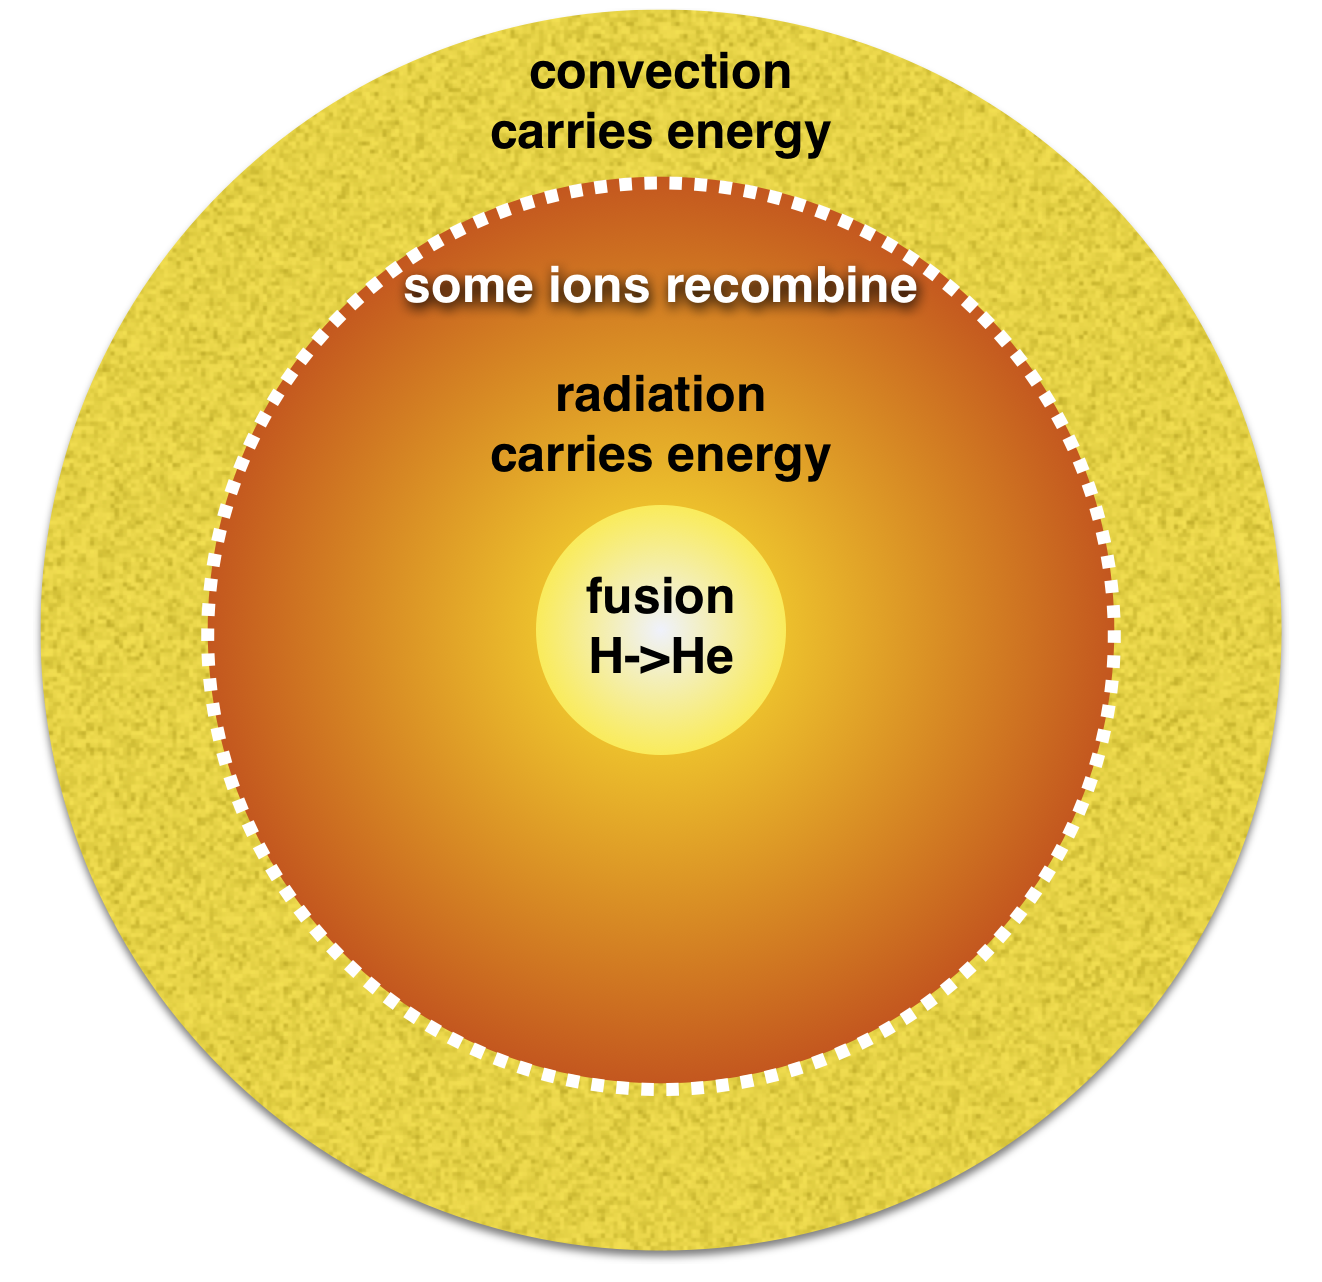
\includegraphics[width=0.75\columnwidth]{sun_structure.png}
\end{figure}
}

\frame{\frametitle{The overshooting convection region in the Sun is usually modeled by looking at variations in density stratification.}
\begin{figure}[h]
	\centering
		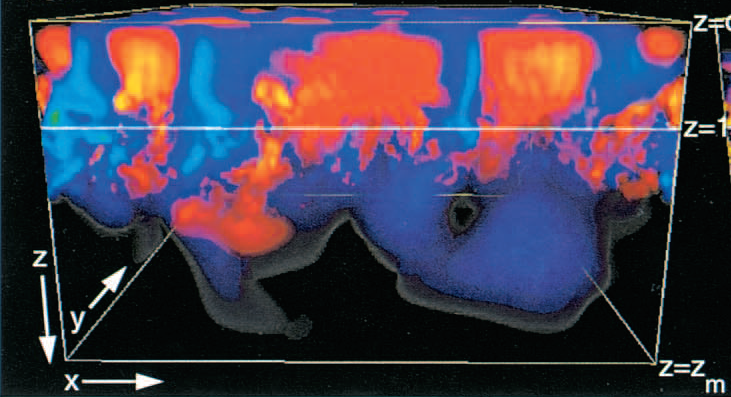
\includegraphics[width=.9\textwidth]{os_image.png}\footnote{\citep{Brummell2002}}
	\label{fig:figs_scdiagram}
\end{figure}
}

\frame{\frametitle{Recall that the condition for convection depends both on the stratification and on the diffusivity.}
\begin{equation}
	Ra\equiv\frac{\alpha g}{\nu \kappa_{T}}\Delta T H^{3}
\end{equation}
and the condition for convection is
\begin{equation}
	Ra>Ra_{\mathrm{crit}}=\mbox{constant based on geometry},
\end{equation}
however, there have been many fewer studies of boundaries due to changes in diffusion.
}

\frame{\frametitle{The overshooting region in the Sun is actually due to a substantial decrease in diffusivity due to ion recombination.}
\begin{figure}
	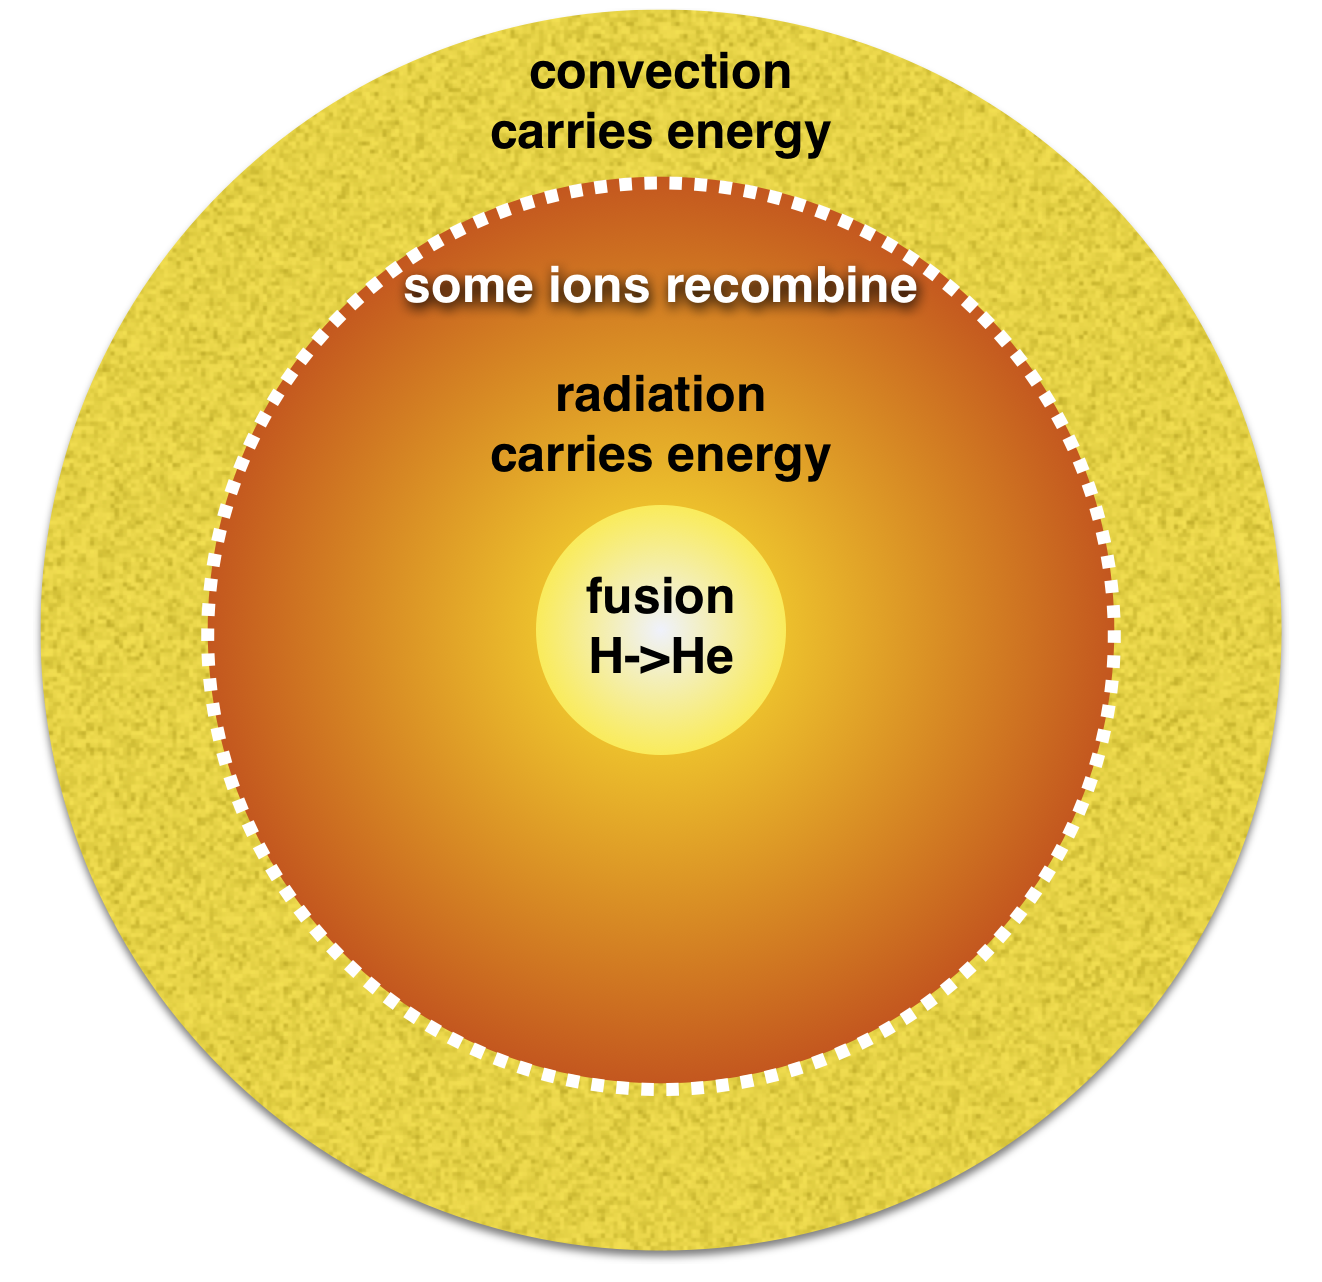
\includegraphics[width=0.75\columnwidth]{sun_structure.png}
\end{figure}
}

\frame{\frametitle{The Sun is a relatively simple star compared to late stage massive stars, which can have quite interesting interiors.}
\begin{figure}
	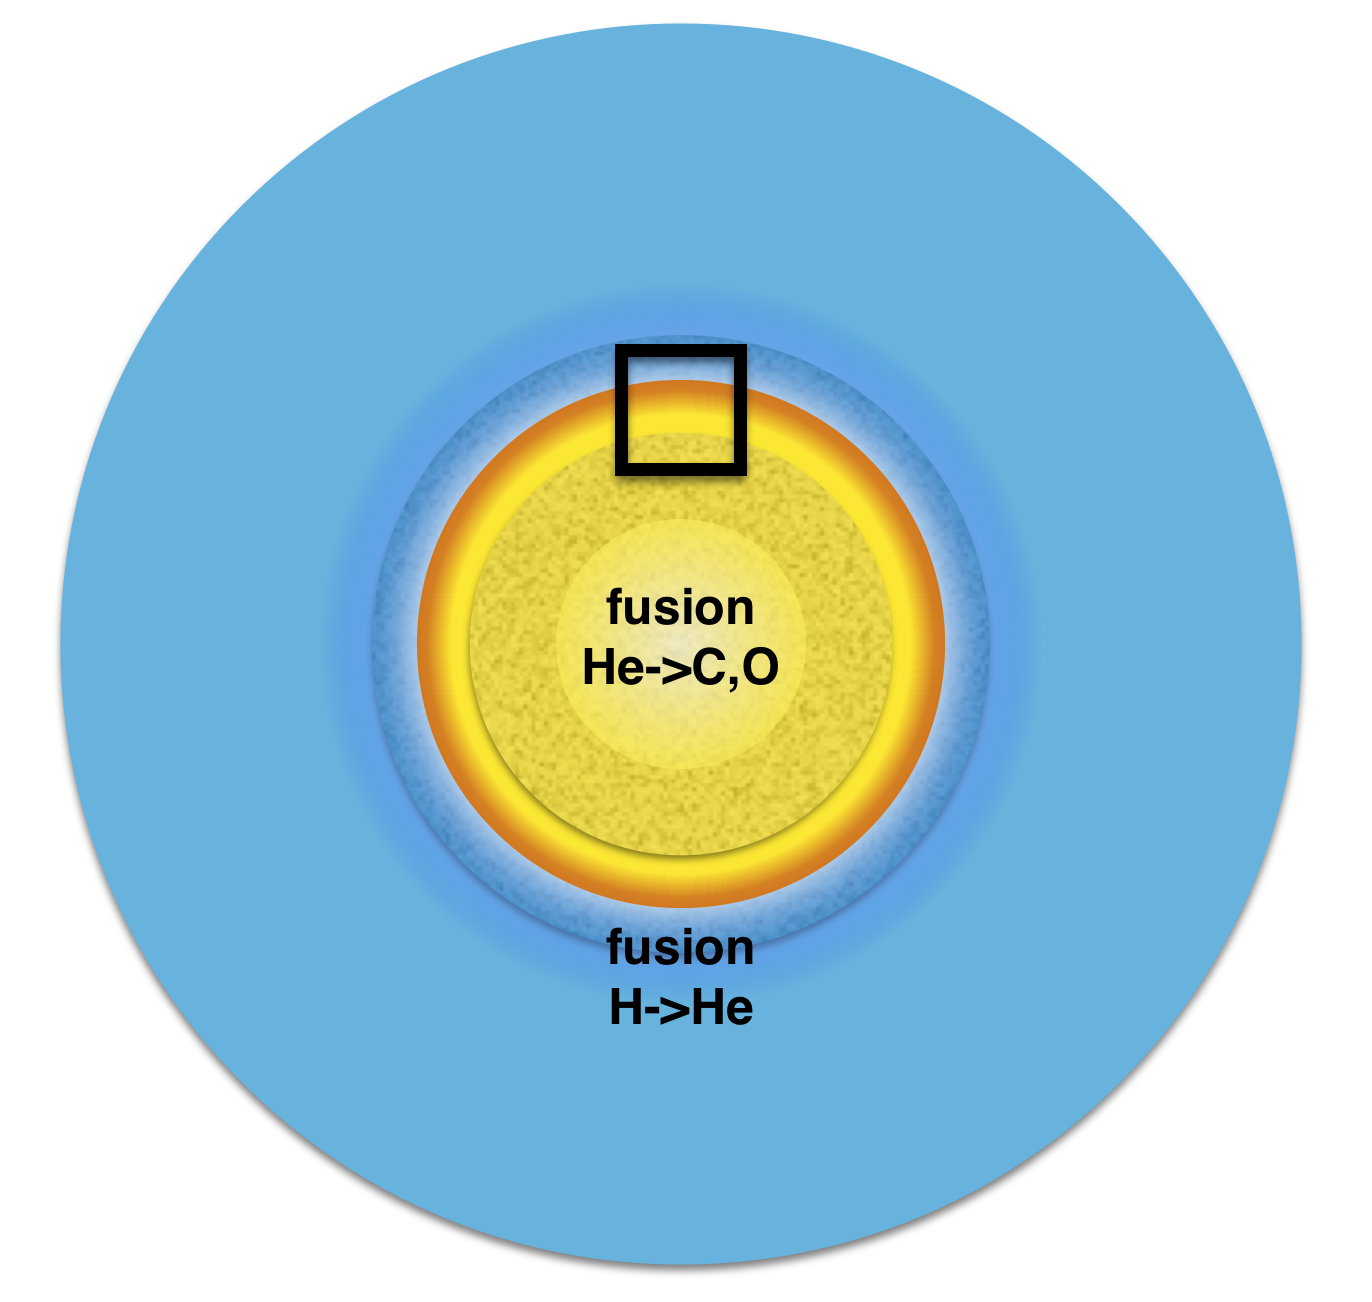
\includegraphics[width=0.75\columnwidth]{bsg_structure.png}
\end{figure}
}

\frame{\frametitle{In this small region, we have many interesting mixing phenomenon all of major importance to the development of the star.}
\begin{figure}
	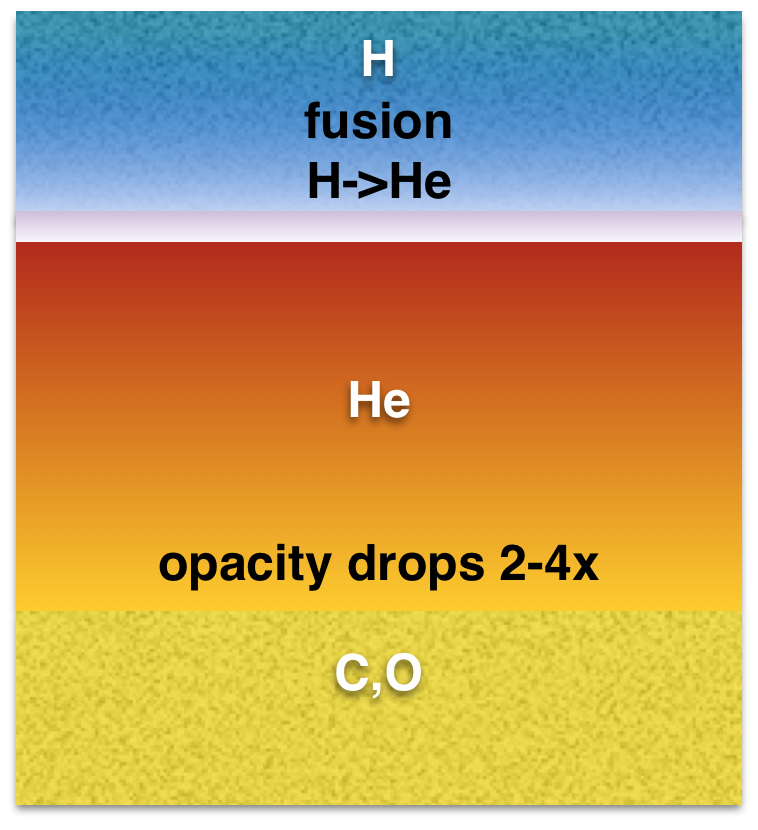
\includegraphics[width=0.5\columnwidth]{bsg_inset.png}
\end{figure}
}

\frame{\frametitle{We'd like a code that can handle:}
\begin{itemize}
	\item Tracking sharp interfaces with high resolution (FC/ODDC)
	\item Spatially-dependent diffusion (OS in Sun/BSG)
	\item Non-linear diffusion for opacity dependence on composition
\end{itemize}
}